\documentclass[12pt]{article}

\usepackage{sbc-template}
\usepackage{graphicx,url}
\usepackage[utf8]{inputenc}
\usepackage[brazil]{babel}
\usepackage{amsmath}
\usepackage{pdfpages}
\usepackage{realboxes}
\usepackage{array}
\usepackage{booktabs}
\usepackage{multirow}
\usepackage{float}
% \usepackage[latin1]{inputenc}  

\graphicspath{ {figures/} }
% \newcommand{\PreserveBackslash}[1]{\let\temp=\\#1\let\\=\temp}
% \newcolumntype{C}[1]{>{\PreserveBackslash\centering}p{#1}}
% \newcolumntype{R}[1]{>{\PreserveBackslash\raggedleft}p{#1}}
% \newcolumntype{L}[1]{>{\PreserveBackslash\raggedright}p{#1}}
\newcolumntype{C}[1]{>{\centering\arraybackslash}p{#1}}
\newcolumntype{R}[1]{>{\raggedleft\arraybackslash}p{#1}}
\newcolumntype{L}[1]{>{\raggedright\arraybackslash}p{#1}}


\sloppy
\raggedbottom

\begin{document} 

\nocite{ChromeV8,Node.js,NPM,ElectronJS}


\includepdf[pages=-]{cover.pdf}

\section{Resumo}

Lorem Ipsum

\newpage

% Indexes

\listoffigures
\listoftables

\newpage

\tableofcontents

\newpage

\section{Introdução}
\subsection{Contextualização: Mercado Financeiro e Negociação de Ações} \label{sec:Stockmarket}

Falar de trabalhos passados. Falar de Preços de Ações. 

\subsubsection{Gráficos OHLC (\textit{Open-High-Low-Close})} \label{sec:OHLC}

A visualização do preço de uma \textbf{ação} normalmente é feita durante quatro momentos
de um período: preço de abertura . os
preços máximo, mínimo, de fechamento e de abertura dentro de um período de tempo,
o período de tempo onde estes preços foram observados, e o volume de ações negociadas
durante o período para uma determinada ação durante um determinado período de tempo.
Estes dados estão contidos em um arquivo .CSV (\textit{comma separated values}).
O programa Metatrader 5, assim como outros sistemas de análise de preços, é capaz de
exportar os preços observados de uma dada ação organizados no formato .CSV de forma
compatível ao uso neste sistema.

\subsection{Motivação: Ondas de Elliott} \label{sec:Elliott-Waves}

Citar limitações de repetibilidade de Elliott e subjetividade.

\section{Extensões de Neely} \label{sec:Neely-Extensions}

Lorem Ipsum Neely...

\subsection{Limitação de Janela de Análise}

Principal limitação das Extensões de Neely: número fixo de pontos na janela de análise
baseadas em uma folha de papel.

\section{Fatores de Estudo}

As Extensões de Neely não especificam algumas configurações que podem alterar a
análise resultante. O preço a ser utilizado é definido por Neely como sendo o de Negociação
(\textit{Cash Market}). Neely cita que Mercados de Negociação costumam gerar uma única cotação
por dia, e essa cotação deve ser usada para compor as análises. Porém, Neely também cita
que alguns Mercados de Negociação operam continuamente, e que nesses casos, uma opção é
escolher um período de tempo para a análise, e usar a média entre o máximo e mínimo do período.\\

Uma ressalva feita por Neely é de que mercados internacionais devem ser observados somente
durante o período em que o mercado está aberto no país onde se está fazendo a negociação.

\begin{itemize}
	\item Preço da Ação
	\begin{itemize}
		\item Média Agregada (HLC)
		\item Mediana (HL)
		\item Preço de Fechamento (C)
	\end{itemize}
	\item Atualização da Regra de Neutralidade (manter atual, não usar, testar nova)
	\begin{itemize}
		\item Atualiza fator a cada novo Movimento Direcional
		\item Não atualizar fator
		\item Não usar Regra de Neutralidade
	\end{itemize}
	\item Escala de Tempo
	\begin{itemize}
		\item Todas as escalas devem usar mesma configuração?
		\item Escalas diferentes usam configurações diferentes?
	\end{itemize}
\end{itemize}

Após a finalização do algoritmo, serão feitas análises de ações com diferentes configurações,
e serão observadas as diferenças nos resultados obitidos para cada configuração.
O objetivo destes testes será analisar o efeito e impacto de cada configuração sobre a
análise resultante.

\newpage

\section{Arquitetura}

Nesta seção será descrita a arquitetura do programa que implementa o algoritmo estudado.

\subsection{Contexto do Sistema}

Um programa capaz de implementar a classificação das Ondas de Elliott de forma consistente
e repetível pode se tornar uma forte ferramenta na análise de variações de preços de ações
no mercado financeiro. A característica programática das Extensões de Neely tornam o método
de Elliott-Neely um ótimo candidato para elaboração de um sistema de análise das
variações de preços de ações no mercado financeiro.

\subsection{Requerimentos}

Nesta seção são delineados os requerimentos para o sistema a ser implementado.
Inicialmente, a visão arquitetural e as partes interessadas são apresentadas, seguidas dos
requerimentos de alto nível e casos de uso. Finalmente, os requerimentos funcionais,
não-funcionais e evolutivos são apresentados.

\subsubsection{Visão arquitetural}

Nesta parte os principais conceitos arquiteturais serão destacados e explicados.\\

A entrada utilizada no sistema são os preços de \textbf{ações}, explicados na Seção
\ref{sec:OHLC}. O sistema atualmente utiliza os dados exportados de outros softwares
em um arquivo .CSV (\textit{comma separated values}), porém há planos de configurar
o programa para obter os dados atualizados em tempo real.\\

A \textbf{interface gráfica} é a parte da aplicação através da qual o usuário final interage
com o sistema e acessa suas funcionalidades.\\

O \textbf{algoritmo Elliott-Neely} é a parte crítica do sistema, sendo a principal responsável
pela análise dos preços de ações alimentadas no sistema. O algoritmo é discutido na Seção
\ref{sec:Neely-Extensions} e sua implementação programática é o objeto de estudo deste
Mestrado.\\

O \textbf{relatório final} é o resultado da análise fornecida pelo sistema. Ele será
implementado na forma gráfica, em notações de Elliott explicadas na Seção
\ref{sec:Elliott-Waves}. Caso a conclusão do algoritmo seja antecipada ao cronograma,
será implementada e emissão de um relatório escrito.

\subsubsection{\textit{Stakeholders}}

O \textbf{usuário final} é o pesquisador/analisador de mercado interessado em realizar uma
análise das Ondas de Elliott nos preços de uma ação do mercado financeiro. Seus interesses são
obter uma resultado confiável dos dados analisados e conseguir utilizar o sistema sem grandes
dificuldades.\\

O \textbf{desenvolvedor} é um pesquisador/programador interessado em atualizar e/ou modificar
o sistema, podendo por exemplo, adicionar novos métodos de análise. Seus interesses são a
manutenibilidade do sistema e a testabilidade do sistema e de seus elementos.\\

A Tabela \ref{tab:stakeholders} mostra a distribuição dos interesses de cada 
\textit{stakeholder}, assim como o interesse total de cada atributo do sistema. Cada
\textit{stakeholder} é igualmente importante, então, cada um recebe 100 pontos para distribuir
entre seus interesses.

\begingroup
\renewcommand*{\arraystretch}{2}
\begin{table}[H]
	\centering
	\caption{Representação Quantitativa dos Interesses dos \textit{Stakeholders}}
	\label{tab:stakeholders}
	\begin{tabular}{ L{4cm} | C{1cm} C{1cm} C{1cm} C{1cm} }
		\textbf{Stakeholders} & 
		\rotatebox{90}{\textbf{Confiabilidade}\hspace{2pt}} &
		\rotatebox{90}{\textbf{Manutenibilidade}\hspace{2pt}} &
		\rotatebox{90}{\textbf{Usabilidade}\hspace{2pt}} &
		\rotatebox{90}{\textbf{Testabilidade}\hspace{2pt}} \\
		\hline
		\textbf{Usuário Final}	&  80 &     &  20 &     \\
		\textbf{Desenvolvedor}	&  30 &  40 &     &  30 \\
		\hline
		\textbf{Total}			& 110 &  40 &  20 &  30 \\
	\end{tabular}	
\end{table}
\endgroup

\subsubsection{Atributos de Qualidade}

Os atributos chaves de qualidade são aqueles que concentram o maior interesse dos
\textit{stakeholders} (Tabela \ref{tab:stakeholders}).\\

\textbf{Confiabilidade} é o atributo chave deste sistema. Por ser um sistema de análise de dados,
a confiabilidade dos resultados está diretamente ligada a qualidade do sistema em si.\\

\textbf{Manutenibilidade} é um atributo secundário deste sistema. A medida que novos
pesquisadores se interessem no sistema, a facilidade de extensão, otimização e manutenção
se toram chaves em manter o interesse dos novos desenvolvedores.\\

\textbf{Testabilidade} permitirá que desenvolvedores tenham mais confiança a cerca do sistema
e das modificações feitas nele.\\

\textbf{Usabilidade} facilitará a interação dos usuários com o sistema.

\subsubsection{Requerimentos de Alto-Nível}

Os seguintes requerimentos representam as funcionalidades de alto-nível do sistema.
Cada requerimento de alto-nível será refinado em detalhe por vários requerimentos específicos
e técnicos.

\begingroup
\renewcommand*{\arraystretch}{1.5}
\begin{tabular}{|p{1cm} p{1cm} p{9cm}|}
	\hline
	\multicolumn{3}{|l|}{\textbf{Análise de Dados}}\\
	HL-1 & Deve &	O sistema deve fazer uma análise das Ondas de Elliott de acordo com as
					Extensões de Neely de forma confiável.\\
	\hline
\end{tabular}

\begin{tabular}{|p{1cm} p{1cm} p{9cm}|}
	\hline
	\multicolumn{3}{|l|}{\textbf{Configuração da Análise}}\\
	HL-2 & Deve &	O sistema deve permitir a mudança da configuração da análise a ser
					feita sobre os dados.\\
	\hline
\end{tabular}

\begin{tabular}{|p{1cm} p{1cm} p{9cm}|}
	\hline
	\multicolumn{3}{|l|}{\textbf{Exibição de Resultados}}\\
	HL-3 & Deve &	O sistema deve exibir os resultados da análise de forma legível para
					o usuário.\\
	\hline
\end{tabular}
\endgroup

\subsubsection{Casos de Uso}

O diagrama de casos de uso é ilustrado na Figura \ref{fig:uc_diagram}, demonstrando os mais
importantes casos de uso e seus atores.

\begin{figure}[H]
	\centering
	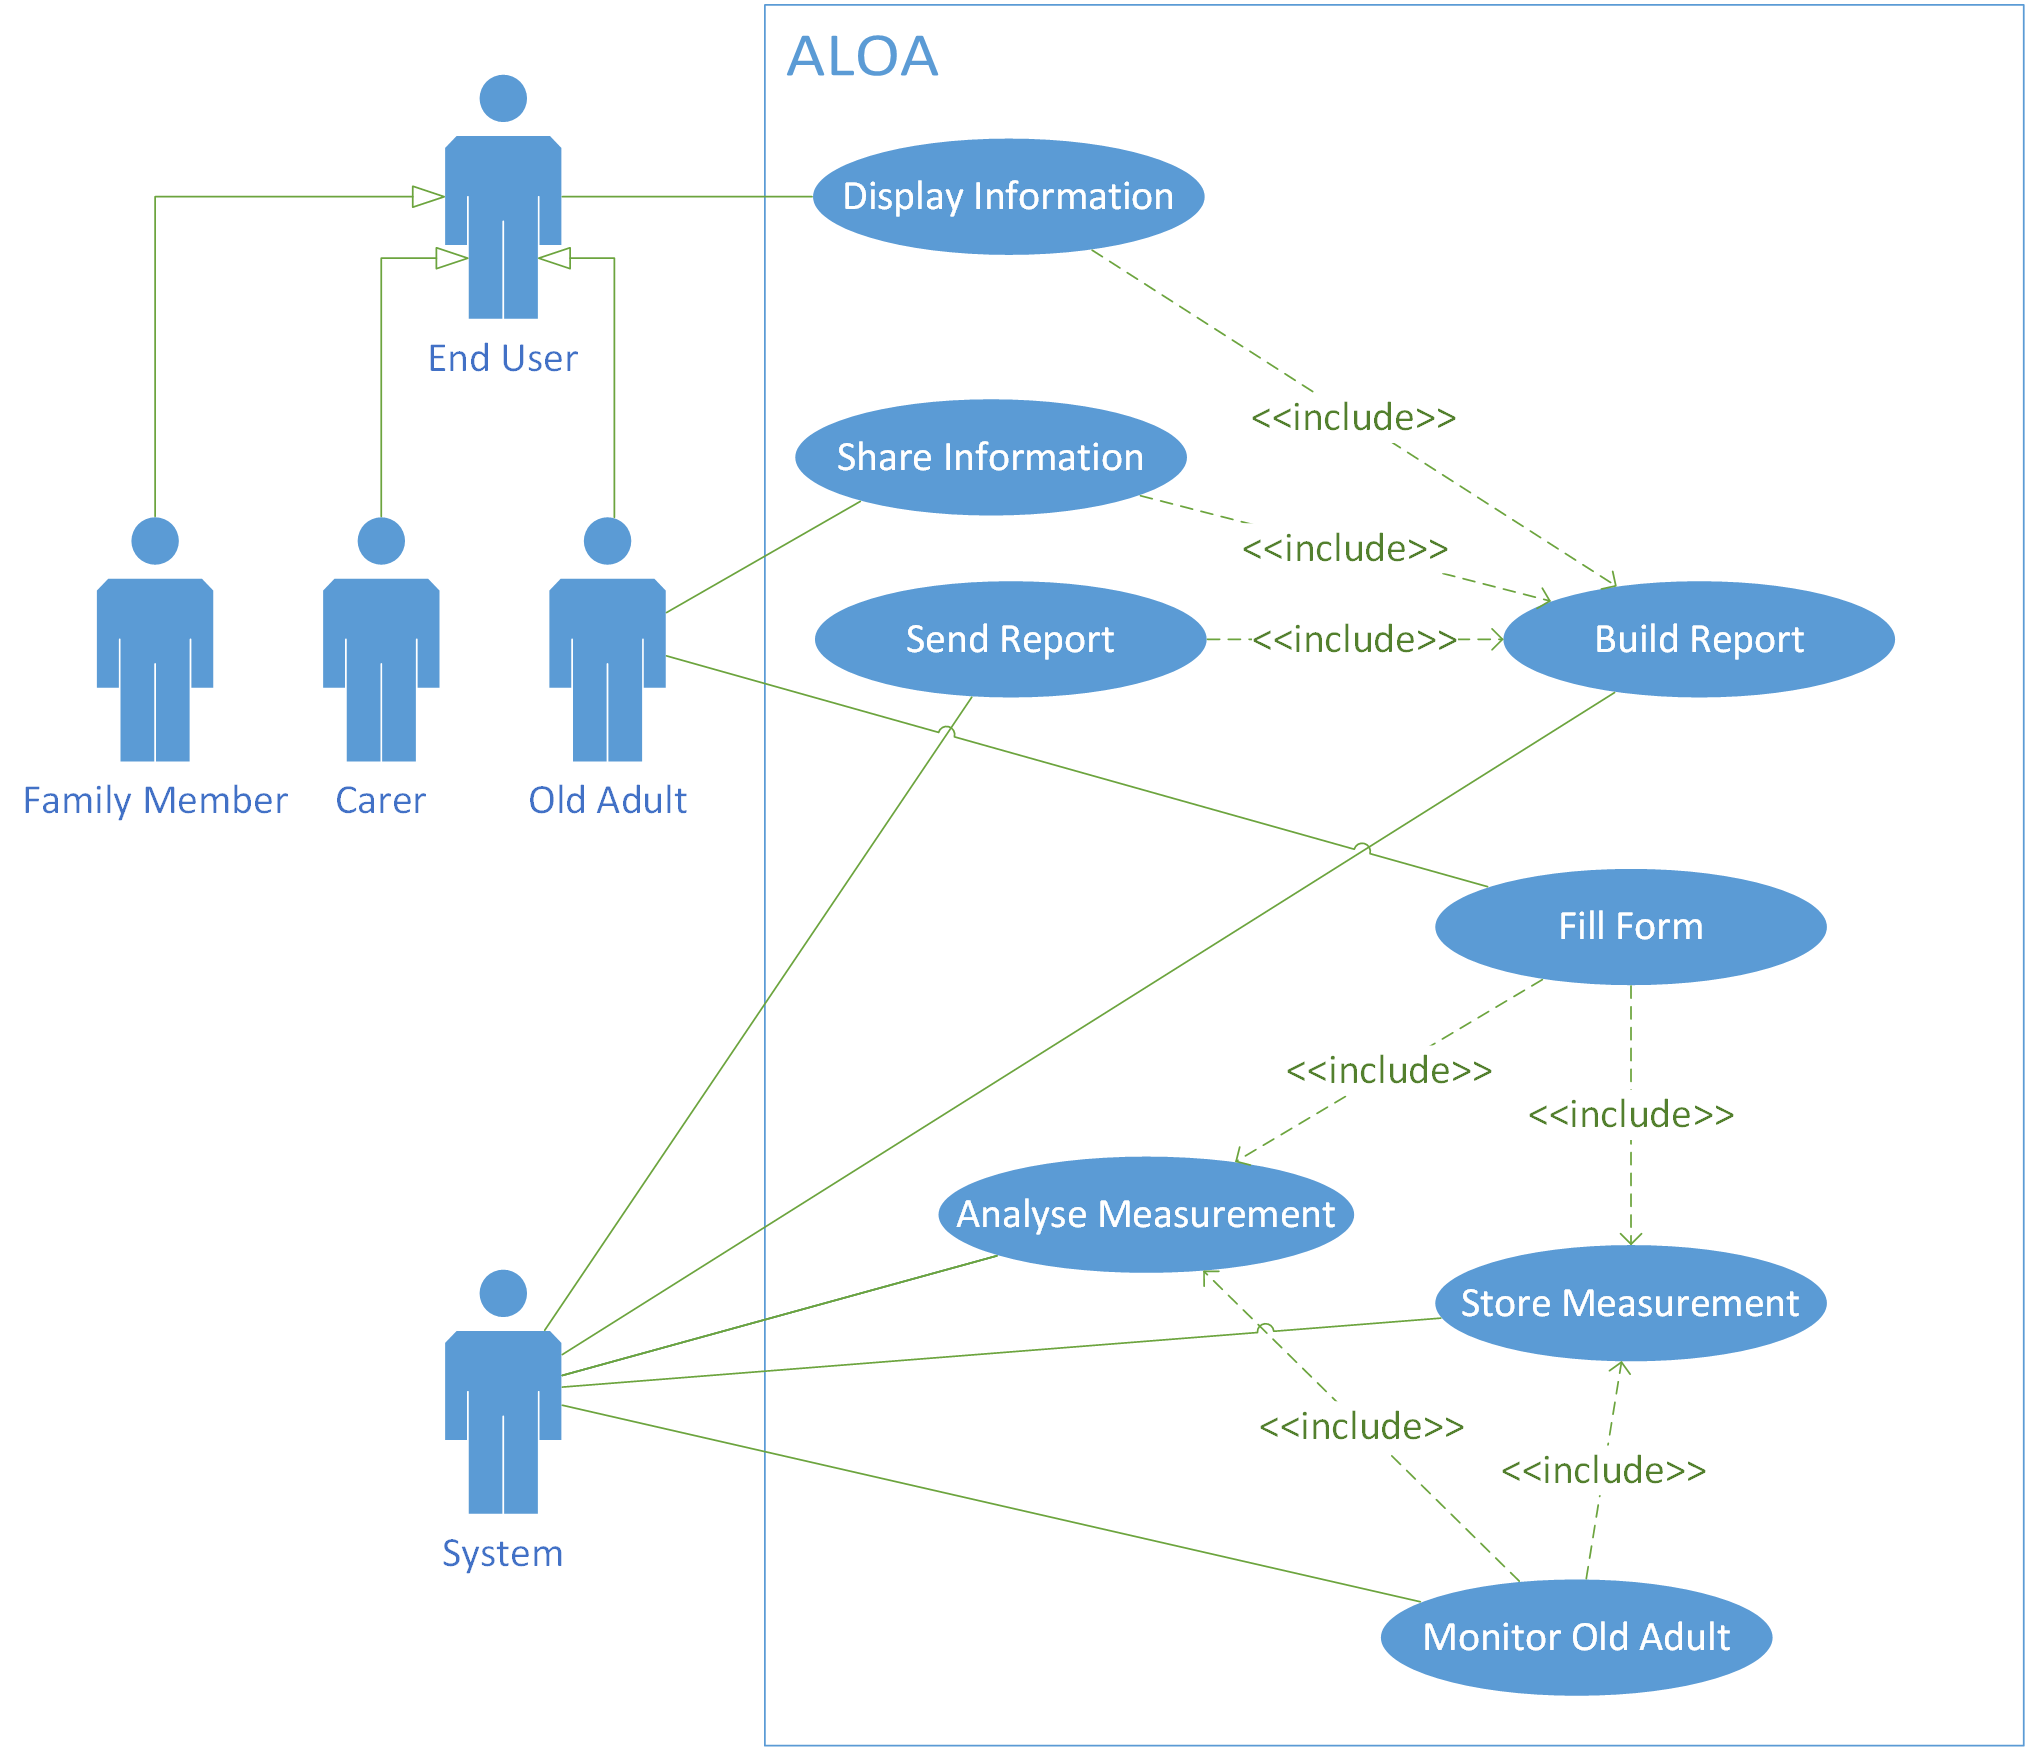
\includegraphics[width=0.5\textwidth]{uc_diagram.png}
	\caption{Diagrama de Casos de Uso}\label{fig:uc_diagram}
\end{figure}

Além disso, as Tabelas a seguir mostram os casos de uso arquiteturalmente significantes.
A numeração refere-se ao requerimento de Alto-nível, por exemplo, UC-1.x refere-se a HL-1.

\begingroup
\renewcommand*{\arraystretch}{1.2}
\begin{table}[H]
	\caption{UC-1.1 - Análise de um Histórico uma Ação}
	\begin{tabular}{p{6cm} p{8cm}}
		\multicolumn{2}{l}{\large{\textbf{UC-1.1 - Análise de um Histórico uma Ação}}}\\
		\toprule
		\textbf{Ator Primário}		&	Usuário Final \\
		\midrule
		\textbf{Objetivo}			&	Analisar o Histórico de uma Ação \\
		\midrule
		\textbf{Condições Iniciais}	&	O sistema está operacional, e o usuário final possui
										o arquivo com o histórico da Ação a ser analisada \\
		\midrule
		\textbf{Cenário Principal de Sucesso}	& \\
		& \begin{enumerate}
			\item O usuário clica na opção de Inserir o Arquivo .CSV com os dados da Ação
			\item O usuário localiza o arquivo .CSV a ser analisado
			\item O sistema valida o arquivo .CSV
			\item O sistema realiza a análise do histórico de preços da Ação
		\end{enumerate}\\
		\midrule
		\textbf{Extensões}	& \\
		& \begin{enumerate}
			\item[3.a] O sistema identifica que o arquivo .CSV não tem as colunas necessárias
			\begin{enumerate}
				\item[3.a.1] O sistema não analisa o arquivo .CSV
				\item[3.a.2] O sistema emite um aviso de que o arquivo .CSV não é válido
				\item[3.a.3] O usuário obtém um arquivo .CSV válido
				\item[3.a.4] Ir para o passo 1 
			\end{enumerate}
		\end{enumerate}\\
		\midrule
		\textbf{Sub-variações} & \\
		& \\
		\midrule
		\textbf{Condições Finais} & O histórico de preços da ação é analisado e o usuário final
									pode alterar as configurações de análise. \\
		\midrule
		\textbf{Requerimentos Relacionados} & HL-1, FR-1, FR-2 \\
		\bottomrule
	\end{tabular}		
\end{table}

\begin{table}[H]
	\caption{UC-1.2 - Mudança na Configuração de Análise}
	\begin{tabular}{p{6cm} p{8cm}}
		\multicolumn{2}{l}{\large{\textbf{UC-1.2 - Mudança na Configuração de Análise}}}\\
		\toprule
		\textbf{Ator Primário}		&	Usuário Final \\
		\midrule
		\textbf{Objetivo}			&	Alterar as configurações de análise \\
		\midrule
		\textbf{Condições Iniciais}	&	Um arquivo válido foi analisado pelo sistema (UC-1.1)\\
		\midrule
		\textbf{Cenário Principal de Sucesso}	& \\
		& \begin{enumerate}
			\item O usuário altera uma das configurações disponíveis na interface
			\item O sistema atualiza a análise de acordo com as novas configurações
		\end{enumerate}\\
		\midrule
		\textbf{Extensões}	& \\
		& \\
		\midrule
		\textbf{Sub-variações} & \\
		& \\
		\midrule
		\textbf{Condições Finais} & A análise é atualizada para a nova configuração. \\
		\midrule
		\textbf{Requerimentos Relacionados} & HL-1, HL-2, FR-3\\
		\bottomrule
	\end{tabular}		
\end{table}

\begin{table}[H]
	\caption{UC-3.1 - Exibição do Resultado da Análise}
	\begin{tabular}{p{6cm} p{8cm}}
		\multicolumn{2}{l}{\large{\textbf{UC-3.1 - Exibição do Resultado da Análise}}}\\
		\toprule
		\textbf{Ator Primário}		&	Sistema \\
		\midrule
		\textbf{Objetivo}			&	Exibir o resultado da análise feita \\
		\midrule
		\textbf{Condições Iniciais}	&	Um arquivo válido foi analisado pelo sistema (UC-1.1)
										ou o usuário alterou as configurações de análise
										(UC-2.1)\\
		\midrule
		\textbf{Cenário Principal de Sucesso}	& \\
		& \begin{enumerate}
			\item O sistema deve exibir o gráfico do histórico do preço da Ação
			\item O sistema deve sobrepor a este gráfico as notações das Ondas de Elliott
		\end{enumerate}\\
		\midrule
		\textbf{Extensões}	& \\
		& \\
		\midrule
		\textbf{Sub-variações} & \\
		& \\
		\midrule
		\textbf{Condições Finais} & O resultado a análise é visível para o usuário final. \\
		\midrule
		\textbf{Requerimentos Relacionados} & HL-3, FR-4 \\
		\bottomrule
	\end{tabular}		
\end{table}
\endgroup

\subsubsection{Requerimentos Funcionais}

Nesta seção, os requerimentos que capturam o comportamento esperado do sistema serão
apresentados (Tabela \ref{tab:functional-requirements}). Este comportamento pode ser
expresso como serviços, tarefas ou funções que o sistema deve executar.
Estes são derivados a partir dos requerimentos de Alto-nível e dos casos de uso.

\begingroup
\renewcommand*{\arraystretch}{1.2}
\begin{table}[H]
	\caption{Requerimentos Funcionais}
	\label{tab:functional-requirements}
	\begin{tabular}{p{1cm} p{1cm} p{12cm}}
		FR-1 & Deve & O sistema deve validar se a entrada é válida.\\
		\midrule
		FR-2 & Deve & O sistema deve informar o usuário caso a entrada seja inválida.\\
		\midrule
		FR-3 & Deve & O sistema deve atualizar automaticamente a análise quando o usuário
					  alterar as configurações.\\
		\midrule
		FR-4 & Deve & O sistema deve realizar a análise automaticamente, e exibir o resultado
					  ao usuário automaticamente.\\
	\end{tabular}		
\end{table}
\endgroup

\subsection{Análise}

Esta seção foca em esclarecer o processo de desenvolvimento do sistema. Aqui, todas as
suposições que são relevantes ao processo são mostradas, assim como o roteiro tecnológico de
desenvolvimento e as decisões de alto-nível tomadas durante o projeto.

\subsubsection{Suposições}

\begin{itemize}
	\item O usuário final tem conhecimento sobre o mercado de ações (Seção \ref{sec:Stockmarket});
	\item O usuário final tem conhecimento sobre a representação dos preços de ações (Seção \ref{sec:OHLC});
	\item O usuário final tem conhecimento sobre as Ondas de Elliott (Seção \ref{sec:Elliott-Waves});
	\item O usuário final tem a sua disposição um software capaz de exportar os preços da
		  ação que quer analisar em formato .CSV;
\end{itemize}

\subsubsection{Roteiro tecnológico}

A primeira versão do sistema foi desenvolvida somente para gerar a representação gráfica
do histórico de preços, e implementar mudanças de configurações básicas. Esta versão teve
como objetivo demonstrar que o ambiente de desenvolvimento era favorável e compatível
com a aplicação a ser criada.\\

A segunda versão do sistema está sendo desenvolvida para implementar a análise de preços
de ações no mercado financeiro conforme o método de Elliott-Neely. Esta versão será capaz
de realizar uma análise das Ondas de Elliott de forma automática, com mínima ou nenhuma
intervenção do usuário.\\

Versões futuras do sistema serão capazes de realizar previsões futuras dos preços das ações,
a partir primariamente da verificação dos padrões das Ondas de Elliott.

\subsubsection{Decisões de Projeto}

As decisões de alto-nível tomadas durante o projeto podem ser vistas nas Tabelas seguintes.

\begingroup
\renewcommand*{\arraystretch}{1.2}
\begin{table}[H]
	\caption{Decisão - Linguagem de Implementação}
	\begin{tabular}{p{3cm} p{11cm}}
		\textbf{Nome}		&	Linguagem de Implementação \\
		\toprule
		\textbf{Decisão}	&   \\
							& 1 \\
		\toprule
		\midrule
		\textbf{Estado}		& Aprovada \\
		\midrule
		\textbf{Problema}	& Qual linguagem de programação utilizar para implementar o algoritmo\\
		\midrule
		\textbf{Decisão}	& Electron (\textit{framework}) + JavaScript (lógica)
							  + HTML5 \& CSS (interface)\\
		\midrule
		\textbf{Alternativas} & \\
		& \textit{C}, \textit{Java}, \textit{C\#}, \textit{Ruby}, \textit{Python} \\
		\midrule
		\textbf{Argumentos} & \\
		& JavaScript é uma linguagem interpretada, com interpretadores disponíveis em vários
		  sistemas operacionais, muitos destes possuindo código aberto com licenças permissivas
		  (como o Chrome V8).\\
		& Node.js é um \textit{runtime} para JavaScript que implementa uma modificação da engine V8,
		  permitindo a execução de código em JavaScript sem a necessidade de um navegador web.\\
		& NPM é um catálogo de bibliotecas e projetos em JavaScript, reunindo mais de 60 mil
		  módulos, com bilhares de downloads semanais e alto controle de versão para cada módulo.\\
		& Electron é um \textit{framework} que permite a criação de programas em 
		  JavaScript + HTML5 \& CSS capazes de rodar em diversos sistemas operacionais 
		  sem problemas de compatibilidade.\\
		& JavaScript possui tipificação dinâmica de variáveis, o que permite uma maior
		  flexibilidade na criação e manuseio de dados.\\
		& Este ecossistema permite a criação de aplicações altamente flexíveis e compatíveis,
		  com acesso a um grande acervo de bibliotecas e módulos para serem integrados,
		  sem problemas de licenciamento, com alto controle de versão.\\
		\bottomrule
	\end{tabular}		
\end{table}
\endgroup

\subsection{Arquitetura do sistema?}

Lorem Ipsum arquitetura

\newpage

\section{Cronograma e Progressão}

Nesta seção são listadas as atividades previstas para realização do trabalho proposto.
Na Tabela \ref{tab:cronograma} é apresentado o cronograma para estas atividades.
Na Tabela \ref{tab:progresso} são listadas as atividades individuais envolvidas na elaboração
e programação do algoritmo estudado.

\begin{enumerate}
	\item Obtenção dos créditos referentes as disciplinas do Mestrado;
	\item Pesquisa bibliográfica;
	\item Redação da monografia para o Exame Geral de Qualificação;
	\item Exame Geral de Qualificação;
	\item Elaboração do algoritmo proposto e programação;
	\item Geração e execução de casos de testes, e avaliação do sistema;
	\item Análise dos efeitos das configurações sobre os resultados do algoritmo;
	\item Redação final da Dissertação; e
	\item Defesa do Mestrado.
\end{enumerate}

\begingroup
\newcommand{\y}{\rule{13,5pt}{5pt}}
\newcommand{\x}{\hspace*{5pt}}
\setlength{\tabcolsep}{0pt}
\begin{table}[H] \footnotesize
\begin{tabular}{|l|c|c|c|c|c|c|c|c|c|c|c|c|c|c|c|c|c|c|c|c|c|c|c|c|}
  \cline{2-25}
  \multicolumn{1}{l|}{} & \multicolumn{5}{c|}{2018} & \multicolumn{12}{c|}{2019} & \multicolumn{7}{c|}{2020}\\
  \cline{2-25}
  \multicolumn{1}{c|}{\textbf{Atividades}} &

  \rotatebox{90}{Agosto\hspace{2pt}} &
  \rotatebox{90}{Setembro\hspace{2pt}} &
  \rotatebox{90}{Outubro\hspace{2pt}} &
  \rotatebox{90}{Novembro\hspace{2pt}} &
  \rotatebox{90}{Dezembro\hspace{2pt}} &
  \rotatebox{90}{Janeiro\hspace{2pt}} &
  \rotatebox{90}{Fevereiro\hspace{2pt}} &
  \rotatebox{90}{Março\hspace{2pt}} &
  \rotatebox{90}{Abril\hspace{2pt}} &
  \rotatebox{90}{Maio\hspace{2pt}} &
  \rotatebox{90}{Junho\hspace{2pt}} &
  \rotatebox{90}{Julho\hspace{2pt}} &
  \rotatebox{90}{Agosto\hspace{2pt}} &
  \rotatebox{90}{Setembro\hspace{2pt}} &
  \rotatebox{90}{Outubro\hspace{2pt}} &
  \rotatebox{90}{Novembro\hspace{2pt}} &
  \rotatebox{90}{Dezembro\hspace{2pt}} &
  \rotatebox{90}{Janeiro\hspace{2pt}} &
  \rotatebox{90}{Fevereiro\hspace{2pt}} &
  \rotatebox{90}{Março\hspace{2pt}} &
  \rotatebox{90}{Abril\hspace{2pt}} &
  \rotatebox{90}{Maio\hspace{2pt}} &
  \rotatebox{90}{Junho\hspace{2pt}} &
  \rotatebox{90}{Julho\hspace{2pt}} \\

  \hline 

  1. Créditos                        & \y & \y & \y & \y & \y & \y & \y & \y & \y & \y & \y & \y & \x & \x & \x & \x & \x & \x & \x & \x & \x & \x & \x & \x\\ \hline
  2. Pesquisa bibliográfica          & \y & \y & \y & \y & \y & \y & \y & \y & \y & \y & \y & \y & \y & \y & \y & \y & \y & \y & \y & \y & \y & \y & \y & \x\\ \hline
  3. Escrita da qualificação         & \x & \x & \x & \x & \x & \x & \x & \x & \x & \x & \y & \y & \y & \x & \x & \x & \x & \x & \x & \x & \x & \x & \x & \x\\ \hline
  4. Apresentação da qualificação    & \x & \x & \x & \x & \x & \x & \x & \x & \x & \x & \x & \x & \x & \y & \x & \x & \x & \x & \x & \x & \x & \x & \x & \x\\ \hline
  5. Elaboração do programa 		 & \y & \y & \y & \y & \y & \y & \y & \y & \y & \y & \x & \x & \y & \y & \y & \y & \y & \y & \x & \x & \x & \x & \x & \x\\ \hline
  6. Testes 						 & \x & \x & \x & \x & \x & \x & \x & \x & \x & \x & \x & \x & \x & \x & \x & \x & \y & \y & \x & \x & \x & \x & \x & \x\\ \hline
  7. Análise de configurações		 & \x & \x & \x & \x & \x & \x & \x & \x & \x & \x & \x & \x & \x & \x & \x & \x & \x & \x & \y & \y & \y & \x & \x & \x\\ \hline
  8. Escrita da dissertação          & \x & \x & \x & \x & \x & \x & \x & \x & \x & \x & \x & \x & \x & \x & \x & \x & \x & \x & \x & \x & \x & \y & \y & \y\\ \hline
  9. Defesa do mestrado              & \x & \x & \x & \x & \x & \x & \x & \x & \x & \x & \x & \x & \x & \x & \x & \x & \x & \x & \x & \x & \x & \x & \x & \y\\ \hline
\end{tabular}
 \caption{Cronograma de atividades}
 \label{tab:cronograma}
 \normalsize
\end{table}
\endgroup

\newpage

\begingroup
\renewcommand*{\arraystretch}{1.5}
\begin{table}[H]
\scriptsize
\begin{tabular}{|L{3cm}|L{2cm}|L{5cm}|R{1.4cm}|R{1.4cm}|}
	\hline
	\textbf{Tópico} & \textbf{Atividade} & \textbf{Descrição} & \textbf{Progresso} & \textbf{Estimado} \\
	\hline
	\hline
	\textbf{Aquisição de Dados}
		& \textbf{Importação de Dados}
		& 	Importação dos Dados OHLC em arquivos .CSV exportados a partir do Programa Metatrader 5. \newline
			Utilizando a biblioteca \textbf{Papaparse}.
		& 100\%
		& - \\
	\hline
	\textbf{Pré-Tratamento de Dados}
		& \textbf{Passagem dos Dados para Classe OHLCT}
		& Transferência dos dados importados do Metatrader 5 para a \textbf{Classe OHLCT}
		& 100\%
		& - \\
		\cline{2-5}
		& \textbf{Escalas de Tempo}
		&	Replica dados originais em diferentes escalas de tempo. \newline
			Implementados: 1 min, 1 hora, 1 dia. \newline
			Escalável para fácil configuração de novas escalas.
		& 100\%
		& - \\
		\cline{2-5}
		& \textbf{Valor Típico}
		&	Cálculo do Valor Típico sobre o qual a análise será feita. \newline
			Implementados: Valor Agregado (HLC), Mediana (HL). \newline
			Escalável para fácil configuração de novos valores típicos.
		& 100\%
		& - \\
	\hline
	\textbf{Método Elliott-Neely \newline Analise Preliminar \newline (1ª parte)}
		& \textbf{Regra de Neutralidade (1º passo)}
		&	Aplicação da primeira passagem da \textbf{Regra de Neutralidade}. \newline
			Implementado através das \textbf{Classes Monowave} e \textbf{Monowave Vector}.
		& 100\%
		& - \\
		\cline{2-5}
		& \textbf{Regra de Proporção \newline (Seleção da Janela de Análise)}
		&	Atualizada para ambiente digital e alta quantidade de dados. \newline
			Afeta a segunda passagem da \textbf{Regra de Neutralidade} e a \textbf{Regra de Retracement}
		& 100\%
		& - \\
		\cline{2-5}
		& \textbf{Regra de Neutralidade (2º Passo)}
		& Une \textbf{monowaves} e/ou altera início/fim de \textbf{monowaves} de acordo com a \textbf{Regra de Proporção}.
		& 100\%
		& - \\
		\cline{2-5}
		& \textbf{Regra de Observação}
		& Aplicada de forma emergente através da \textbf{Classe Monowave Vector}.
		& 100\%
		& - \\
		\cline{2-5}
		& \textbf{Regra de Retracement}
		& Classificação de \textbf{Monowaves}.
		& 0\%
		& 3 semanas \\
	\hline
	\textbf{Método Elliott-Neely \newline Observações Intermediárias \newline (2ª parte)}
		& \textbf{Regra de Similaridade e Balanço}
		& Indica quais \textbf{Monowaves} pertencem ao mesmo grupo/grau para efeito de agrupamento.
		& 0\%
		& 2 semanas \\
	\hline
	\textbf{Método Elliott-Neely \newline Considerações Centrais \newline (3ª parte)}
		& \textbf{Construção de Polywaves}
		& Classifica conjuntos de \textbf{Monowaves} nos padrões das \textbf{Ondas de Elliott}.
		& 0\%
		& 3-4 semanas \\
		\cline{2-5}
		& \textbf{Extensões de Neely}
		& Aplica regras de compactação que transformam grupos de \textbf{Monowaves} em \textbf{Monowaves} de grau maior.
		& 0\%
		& 3-4 semanas \\
	\hline
	\textbf{Interface com Usuário}
		& \textbf{Visualização em Gráfico}
		& Utilizando a biblioteca \textbf{Plotly.js}
		& 100\%
		& - \\
		\cline{2-5}
		& \textbf{Configurações}
		& Eixo Vertical (Log ou Linear), Eixo Horizontal (Tempo ou Sequencial), Tipo de Marcador (OHLC, Candelstick ou Nenhum), Resolução do Tempo (1 Minuto, 1 Hora, 1 Dia), Valor Típico (HLC ou HL), Monowave (Visualizar ou Esconder)
		& 100\%
		& - \\
	\hline
\end{tabular} 
\caption{Progresso do algoritmo}
\label{tab:progresso}
\end{table}
\endgroup

\newpage

\bibliographystyle{sbc}
\bibliography{report}

\end{document}
